\subsection{Synthetic Experiments}
\label{sec:synth}

In this section we describe our results on extensive synthetic experiments performed with our model and different benchmark methods in two conditions:
1) missing at random views for each dataset,
and 2) datasets with systematically missing views (missing not at random).

%%%%%%%%%%%%%%%%%%%%%%%%%%%
%% SYNTHETIC EXPERIMENTS %%
%%%%%%%%%%%%%%%%%%%%%%%%%%%
\subsubsection{Data preparation}

To simulate multi dataset observations, we sample the latent variable $\z_{d,n}$ from a multivariate Gaussian with zero-mean and identity covariance matrix, and subsequently we transform each sample with random linear mapping towards the observation space to obtain $\xdnv$.
The detailed procedure is described in \asupmat.
We then corrupt the observations with increasing levels of noise
and we finally remove views in the context of the \textit{missing at random} (MAR) and \textit{missing not at random} (MNAR) experiments.

%% MAR %%
In the MAR experiments views were randomly removed according to a parameter $0 \leq f \leq 1$, which controls the fraction of data-points with complete views.
In the limit case $f=1$, each data-point has all the views, representing the ideal case of no missing views, that is the working case of the Multi-Channel Variational Autoencoder \citep{Antelmi2019}.
In the case $f=0$, each data-point has one and only one randomly assigned view, representing the extreme case where no direct relationship between views is observable.
Here our multi-view model collapses into a disjoint series of independent Variational Autoencoders \citep{Kingma2013, Rezende2014}.
In the general case, each data-point has probability $f$ to have all the views, and probability $1-f$ to have a randomly assigned view out of the total available views.
The general case represents the case where the relationship between views can be established only through a fraction $f$ of the total available data-points.

%% MNAR %%
In the MNAR experiments we removed specific views for each simulated dataset, ensuring at the same time the absence of at least one view for a datasets, and the presence of at least one view in common between pairs of datasets.
As an example, in the case with three datasets and three views, the association view-dataset can be expressed through the following association matrix $A$:
\begin{equation}
A = 
\begin{pmatrix}
1 & 0 & 1 \\
1 & 1 & 0 \\
0 & 1 & 1 
\end{pmatrix},
\end{equation}
where $A(v,d)=1$ indicates the presence of view $v$ in dataset $d$.
For experimental purposes we limited our MNAR simulations to cases that can be defined with square association matrices having a dimensionality not greater than $5\times5$.

\subsubsection{Model Fitting and Evaluation}
In both MAR and MNAR experiments we fit the synthetic scenarios with our model, where we choose a linear Gaussian parametrization for variational and likelihood distributions, made explicit respectively in \eqnref{eq:encoder} and \eqnref{eq:decoder}, with a latent dimension matched to the one used to generate the data.
We trained our model for $10000$ epochs which ensured convergence, after setting up the Adam optimizer with a learning rate of 0.001.
For each simulated scenario we predicted the missing views according to \eqnref{eq:reconstruction} on testing hold-out datasets.

Results, cross-validated on $5$ folds, are summarized with the \textit{mean squared error} (MSE) metric on testing hold-out datasets for every simulated scenario.
We applied the same evaluation procedure for the benchmark methods.

\subsubsection{Benchmark Methods}
Among state of the art multivariate linear and non linear imputation methods, we selected the following benchmark approaches:
1) $k$-Nearest Neighbors (KNN) with $k=\set{1, 5}$;
2) Denoising Autoencoder (DAE) \citep{dae};
3) Multivariate Imputation by Chained Equations (MICE) \citep{Vanbuuren2000}.

For the KNN approach we used the \textit{KNNImputer} method as implemented in the \textit{Scikit-Learn} library \citep{sklearn}.
Here each sample's missing values are imputed using the mean value from $k$ nearest neighbors found in the training set, according to their Euclidean distance.
%Two samples are close if the features that neither is missing are close in terms of Euclidean distance.

The Denoising Autoencoder, initially developed by \cite{Vincent2008}, is based on an overcomplete deep autoencoder.
It maps input data to a higher dimensional space which, in combination with an initial dropout layer inducing corruption, makes the model robust to missing data.
We used the same architecture proposed by \cite{dae}, that is three hidden layers for encoder and decoder networks, Tanh activation functions, hyperparameter $\Theta=7$, and dropout $p=0.5$, as they proved to provide consistently better results.

In MICE, as implemented in \cite{mice}, missing values are modeled as a multivariate linear combination of the available features.
This methodology is attractive if the multivariate distribution is a reasonable description of the data, which in our case it is by construction.
MICE specifies the multivariate imputation model on a variable-by-variable basis by a set of conditional densities, one for each incomplete variable.
Starting from an initial imputation, MICE draws imputations by iterating over the conditional densities.

\subsubsection{Results}
\begin{figure}[htb]
\centering
\begin{subfigure}{.49\textwidth}
	\centering
        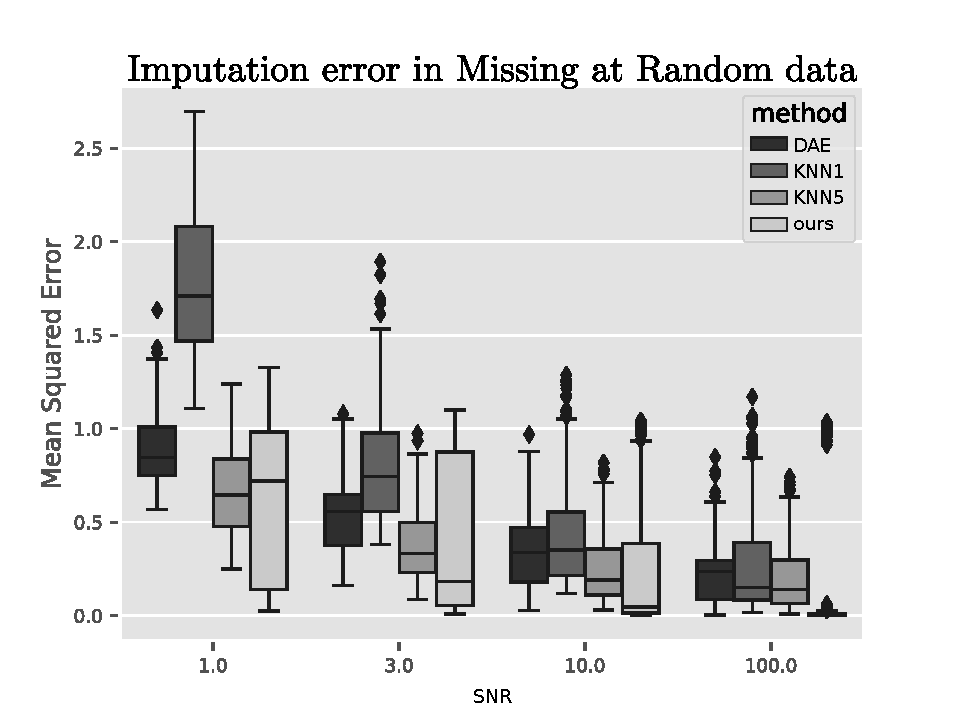
\includegraphics[width=\textwidth]{./tex/fig/mar_imput_err_boxplot.pdf}
        \caption{Missing at random}
        \label{fig:synthetic_benchmark_mar_box}
\end{subfigure}%
\hfill
\begin{subfigure}{.49\textwidth}
	\centering
        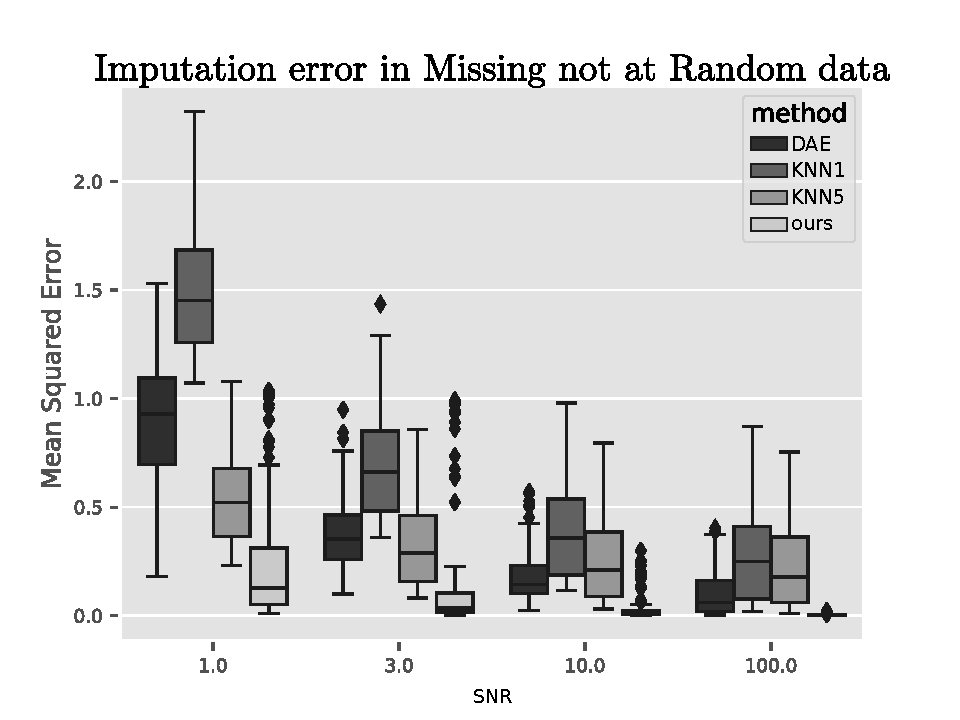
\includegraphics[width=\textwidth]{./tex/fig/mnar_imput_err_boxplot.pdf}
        \caption{Missing not at random}
        \label{fig:synthetic_benchmark_mnar_box}
\end{subfigure}
\caption{
Mean Squared Error of imputation in synthetic datasets. Effect of signal-to-noise ratio (\snr) is shown.
}
\label{fig:synthetic_benchmark_box}
\end{figure}

\begin{figure}[htb]
\centering
\begin{subfigure}{.49\textwidth}
	\centering
        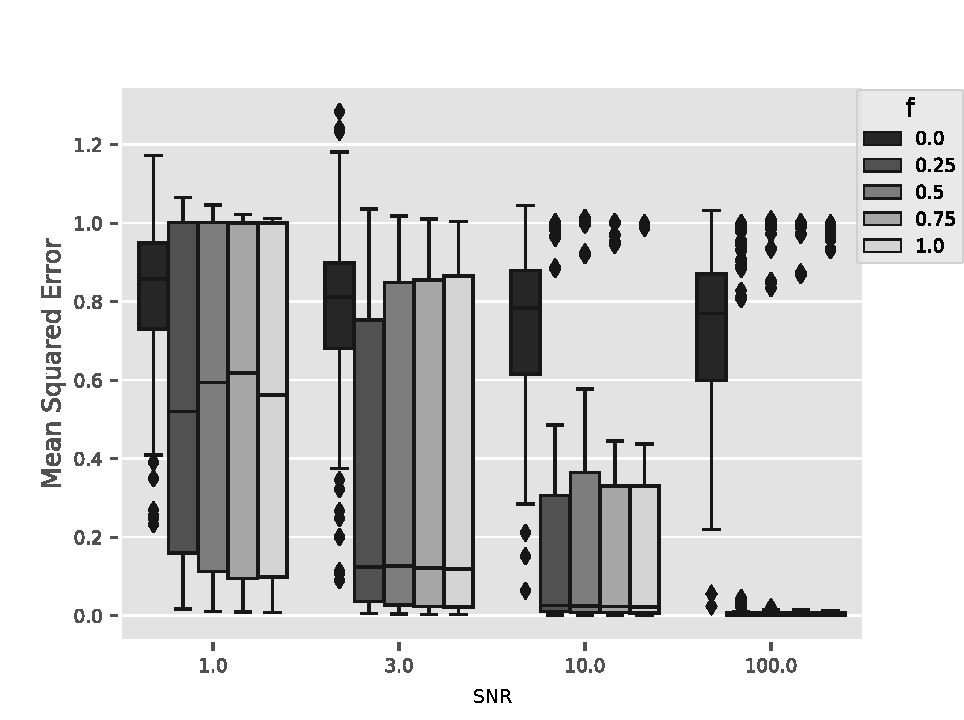
\includegraphics[width=\textwidth]{./tex/fig/mar_pred_err_boxplot.pdf}
        % \caption{Missing at random}
        % \label{fig:synthetic_benchmark_mar_pred_box}
\end{subfigure}%
\caption{
Mean Squared Error of test sets predictions in synthetic datasets.
We show how with already $f \geq 0.25$ (the fraction of observations with all the views) we can significantly reduce the prediction error on testing data-points.
}
\label{fig:synthetic_benchmark_pred_box}
\end{figure}
% \begin{figure}[htb]
% \centering
% \begin{subfigure}{.45\textwidth}
%       \centering
%         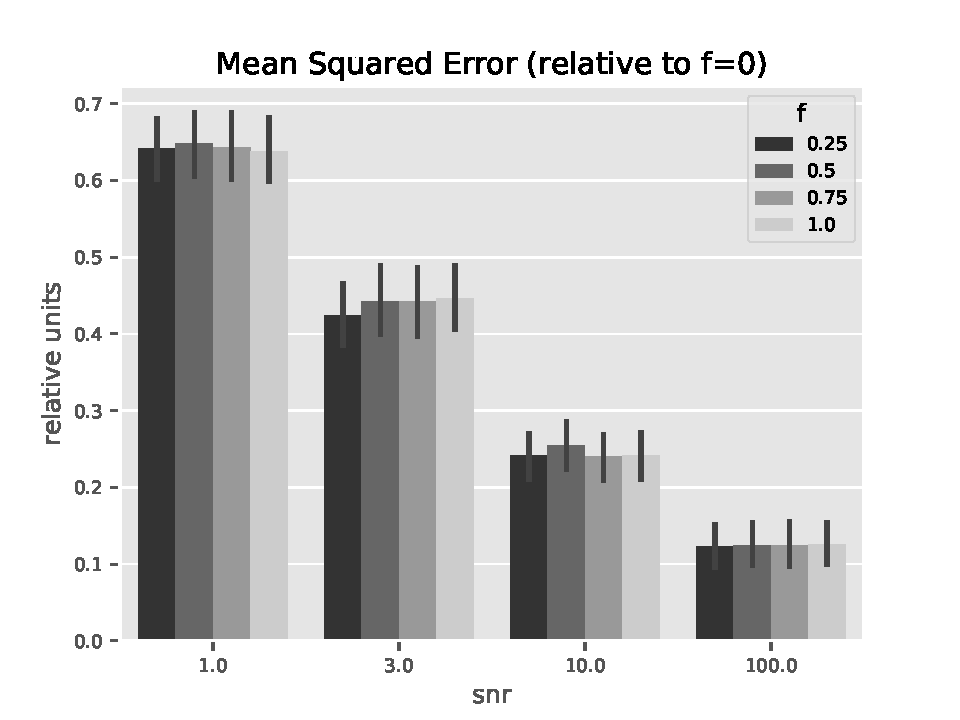
\includegraphics[width=\textwidth]{./tex/fig/mar_barplot.pdf}
%         \caption{Missing at random}
%         \label{fig:synthetic_benchmark_mar_bar}
% \end{subfigure}%
% \hfill
% \begin{subfigure}{.45\textwidth}
%       \centering
%         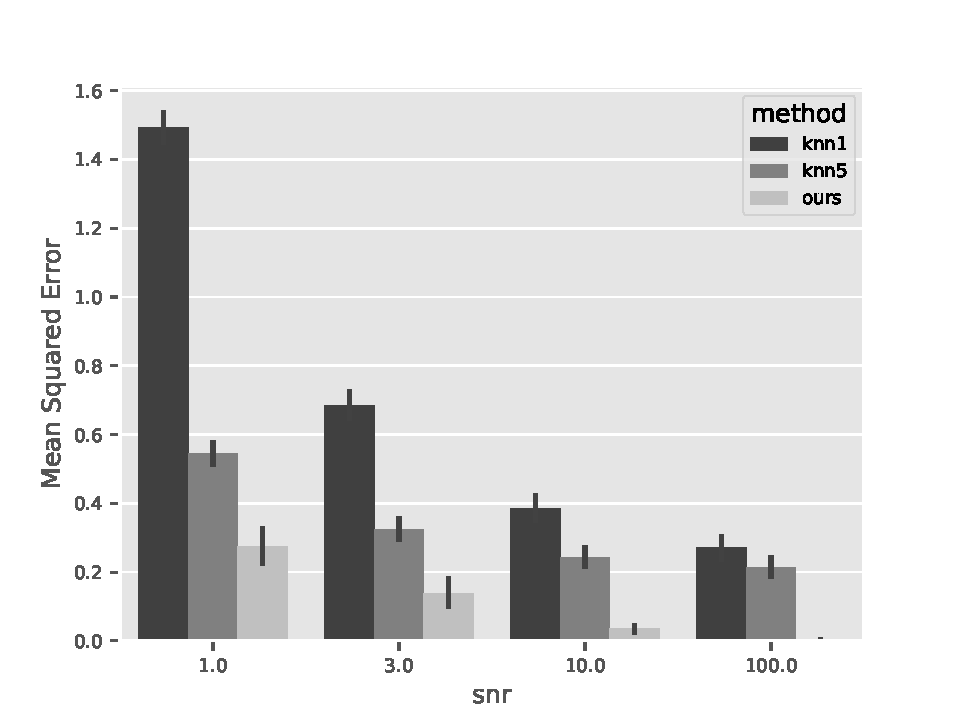
\includegraphics[width=\textwidth]{./tex/fig/mnar_barplot.pdf}
%         \caption{Missing not at random}
%         \label{fig:synthetic_benchmark_mnar_bar}
% \end{subfigure}
% \caption{
% Mean Squared Error of test sets predictions in synthetic datasets. Effect of signal-to-noise ratio (\snr) is shown.
% (a) With $f$ being the fraction of observation with complete views, we show how with already $f \geq 0.25$ we can significantly reduce the prediction error on testing data-points.
% (b) In multi-view datasets where none of the data-point have all the views, and where the available views depends on the specific dataset, we show the prediction performance of our model in comparison with classic k-nearest-neighbors imputation methods.
% }
% \label{fig:synthetic_benchmark_bar}
% \end{figure}



In the synthetic tests our model provides the best performances overall, with a mean MSE improvement compared to the best competing method of $17\%$ in MAR cases and $71\%$ in MNAR cases (\figref{fig:synthetic_benchmark_box}).
%\textcolor{blue}{
%\refnum{\#23}
	We notice that DAE is not always better than KNN ($k=5$), especially in low $\snr$ cases.
%}
%\textcolor{blue}{
%\refnum{\#22}
	We were able to fit the MICE model only on MNAR cases with high $\snr$, where it performed poorly (boxplot not shown), while in all the other cases, including all MAR cases, the model did not converge.
%}

%\textcolor{blue}{
%\refnum{\#10}
	In \figref{fig:synthetic_benchmark_pred_box} we show MAR experiments results stratified by $\snr$ and by the fraction $f$ of data-points with complete views.
	Here we notice how with already $f = 0.25$ we can significantly reduce the prediction error on testing data-points compared to the case $f=0$, where no relationship between views can be established.
	Moreover, reaching the ideal case of $f=1$, that is when there are no missing views in the dataset, does not improve significantly the prediction performance of our model compared to the case $f = 0.25$.
%}
